\documentclass[11pt]{article}
\usepackage[utf8]{inputenc}
\usepackage[ngerman]{babel}

\usepackage{amsmath,amsthm,amssymb,amsfonts}

\usepackage{graphicx}
\usepackage{float}
\usepackage{tikz}

\usepackage{fancyhdr} % For headers and footers
\usepackage{geometry}
\usepackage{listings}
\usepackage{hyperref}
\hypersetup{
    linkcolor=blue,     
    urlcolor=cyan,
}

\geometry{
    a4paper, % Change this if you intend to print on a different paper size, such as letter paper.
    left=20mm,
    right=20mm,
    top=30mm,
    bottom=30mm,
}

\newcount\colveccount
\newcommand*\colvec[1]{
        \global\colveccount#1
        \begin{pmatrix}
        \colvecnext
}
\def\colvecnext#1{
        #1
        \global\advance\colveccount-1
        \ifnum\colveccount>0
                \\
                \expandafter\colvecnext
        \else
                \end{pmatrix}
        \fi
}

\title{Dynamik - Radialkraft (Rotation)}
\author{Emil Staikov}
\date{31. Mai 2021}

\begin{document}
\maketitle
Wenn man einen Ball an einer Schnur dreht, merkt man einen Zug in der Hand, man muss gegenhalten, damit der Ball nicht wegfliegt. Wenn man loslässt, fliegt der Ball mit der Schnur tangential (also entlang der Gerade, die den Kreis in dem Punkt berührt, in dem man loslässt) weg. \\\\


\section{Die Radialkraft}
Ein um eine Achse rotierendes Objekt ändert die ganze Zeit seine Richtung. Da die Geschwindigkeit ein Vektor ist, konstituiert eine Richtungsänderung ebenfalls eine Änderung. In jeder Rotation existiert also eine Beschleunigung (definiert als die Änderung der Geschwindigkeit pro Zeit). Die Kraft, die diese Beschleunigung verursacht, wird als Radialkraft (oft $\vec{F}_r$) bezeichnet, da sie auf den rotierenden Körper stets in Richtung der Drehachse, also entlang des Radius, wirkt. Auf das Objekt, dass die Radialkraft ausübt, wirkt vom rotierenden Objekt aus eine entgegengesetzt gleiche Gegenkraft $-\vec{F}_r$. Das ist \textit{nicht} die Zentrifugalkraft, diese Gegenkraft hat keinen besonderen Namen. 
\begin{figure}[H]
    \centering
    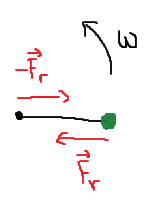
\includegraphics{abb/5-rotation-radialkraft/radialkraft.png}
    \caption{Kräfte bei der Rotationsbewegung. }
\end{figure} 

\noindent Die Radialkraft, die bei einer Rotationsbewegung auf einen um eine Achse rotierenden Körper wirken muss, hat den Betrag 
\begin{equation*}
    |\vec{F}_r| = m\frac{v_T^2}{r} = m\omega^2r
\end{equation*}
Hierbei ist $m$ die Masse, $v_T$ die Tangentialgeschwindigkeit, $\omega$ die Winkelgeschwindigkeit und $r$ der Radius (also der Abstand von der Drehachse) des rotierenden Objekts. Es gilt $v_T = r\omega$. Die Tangentialbeschleunigung $a_r$ ist dann $\frac{v_T^2}{r} = \omega^2r$. \\\\


\section{Beispiele}
In verschiedenen Rotationsbewegungen können verschiedene Kräfte als Radialkraft agieren. In dem zum Anfang angeführten Beispiel üben wir durch das Halten eine Kraft in Größe der Radialkraft auf das Seil aus, welches wiederum eine betraglich gleiche Spannkraft auf den Ball ausübt. Wir merken die Spannkraft am anderen Ende des Seils. Im System Erde-Mond rotiert der Mond um die Erde, eine Kraft muss also als Radialkraft agieren und den Mond auf seiner Bahn halten. Diese Aufgabe erfüllt die Gravitationskraft zwischen Erde und Mond, der Mond übt auf die Erde eine entgegengesetzt gleiche Gegenkraft aus. Fallen euch noch andere Rotationsbewegungen ein? Was sind die zugehörigen Radialkräfte? \\\\ 

Im System Erde-Mond können wir mithilfe der Radialkraft aus der Masse der Erde den Abstand von Erde und Mond ausrechnen. Die hier wirkende Gravitationskraft ist jedoch nicht mehr sinnvoll mit $mg$ zu approximieren, wir rechnen mit dem Newton'schen Gravitationsgesetz
\begin{equation*}
    F_G = G \frac{m_1m_2}{r^2}
\end{equation*}
Die Gravitationskraft zwischen zwei beliebigen Körpern ist proportional zu der Masse der beiden Körper und antiproportional zu ihrem Abstand im Quadrat. Der Proportionalitätsfaktor ist die Gravitationskonstante $G$. Im System Erde-Mond wirkt diese Kraft als Radialkraft, wir können also gleichsetzen: 
\begin{equation*}
    G \frac{m_Mm_E}{r^2} = m_M\omega^2r 
\end{equation*}
Das lässt sich umstellen zu 
\begin{equation*}
    r  = \sqrt[3]{G\frac{m_E}{\omega^2}}
\end{equation*}
$G$ und $m_E$ sind aus dem Tafelwerk abzulesen, $\omega$ folgt aus der Umlaufzeit $T \approx 27d$ des Monds. Setze diese Werte ein, achte auf die Einheiten und vergleiche sie mit einem Buchwert für den Abstand $r$ von Erde und Mond. Wodurch sind Abweichungen zu erklären? 
\end{document}